\begin{longtable} { | c | p{12cm} | c | } 
\hline
	ID 	&	Issues	&		 Es. hours \\\hline
	28 	&	Remove the Childlist	&	32 hours \\\hline
\caption{Issue ID 28}
\label{tab:spr2_removechildlist}
\end{longtable}

It was originally possible to select a child within the application through a menu on the left side of the screen. This was never the intention since the Launcher application handles both the guardian login and which child to work with. As a result, the entire menu has been removed and Sekvens now takes a child as \ct{intent} from the Launcher instead. Figure \ref{fig:withList} and figure \ref{fig:withoutList} is a side by side comparison of the overview with and without the childlist. 

\begin{figure}[ht!]
\centering
\begin{minipage}{.45\textwidth}
\centering
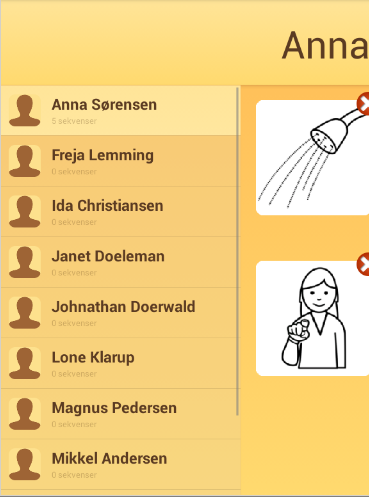
\includegraphics[scale=0.9]{Pics/Sprint2/childlists/withList.png}
\caption{A picture of the overview with a ChildList}
\label{fig:withList}
\end{minipage}\hfill
\begin{minipage}{.45\textwidth}
\centering
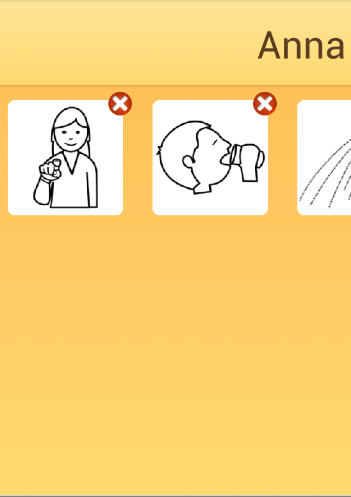
\includegraphics[scale=0.9]{Pics/Sprint2/childlists/withoutList.png}
\caption{A picture of the overview without a ChildList}
\label{fig:withoutList}
\end{minipage}
\end{figure}

